

Pairing lies at the heart of nuclear physics and the quantum
many-body problem in general \cite{ring_nuclear_1980,richardson_restricted_1963,dean_pairing_2003}.
Pairing correlations, the tendency of identical nucleons to form correlated Cooper pairs, play an important role in  nuclear many-body systems.  Soon after the Bardeen–Cooper–Schrieffer (BCS) theory explained electron superconductivity, Bohr, Mottelson, and Pines famously pointed out an analogy in nuclei, namely that nucleons near the Fermi surface couple into Cooper pairs, giving rise to nuclear superfluidity~\cite{bohr_possible_1958}.  Early applications of BCS theory to nuclei demonstrated that including pairing dramatically improves the description of nuclear properties. Indeed, pairing underlies numerous phenomena in finite nuclei, from the extra binding of even-even nuclei to their characteristic excitation spectra. 

In nuclear physics, pairing is treated using models originally inspired by electronic superconductors. The simplest approach is the BCS model \cite{richardson_restricted_1963,bohr_possible_1958}, in which a condensate of nucleon pairs (typically in a spin-singlet, $^1S_0$ state) occupies the nuclear ground state. The BCS theory successfully explained why even-even nuclei are more tightly bound than their odd-$A$ neighbors (the odd–even mass staggering) and why even-even nuclei have an energy gap to the first excited state. However, the standard BCS wave function is not an eigenstate of particle number and it violates the conservation of nucleon number by allowing coherent superpositions of different particle numbers. In the mean-field context, this is remedied by the Hartree–Fock–Bogoliubov (HFB) approach \cite{Dobaczewski2002}, which combines the Hartree–Fock description of single-particle motion with a Bogoliubov transformation to incorporate pairing correlations self-consistently. This approach extends the independent-particle model to a quasiparticle basis, wherein the normal single-particle density and the pairing tensor are determined simultaneously by variational minimization of the energy. This formalism (and its variants within energy density functional theory) is the workhorse for modeling open-shell nuclei and has been applied extensively across the nuclear chart and even to uniform nuclear matter . For example, HFB calculations with effective interactions can predict pairing gaps in nuclei and in neutron-star matter within a unified framework.

Beyond the mean-field level, important refinements to pairing theory have been developed. One class of methods focuses on restoring broken symmetries – in particular, enforcing exact particle-number conservation. 

In finite nuclei, pairing correlations profoundly shape nuclear structure. A primary signature is the odd–even staggering of binding energies: nuclei with an even number of neutrons (and/or protons) are systematically more bound than the interpolating odd-$A$ nuclei, reflecting the energy gain from pairing two like nucleons. Quantitatively, this pairing gap is on the order of $\sim1$–2 MeV in many medium and heavy nuclei, see for example \cite{Dean2003} for examples. Even–even nuclei (with all nucleons paired) exhibit a pairing gap in their excitation spectrum. Here, the lowest excited state requires breaking a Cooper pair. In contrast, neighboring odd-$A$ nuclei (with one unpaired nucleon) have a compressed low-lying spectrum, as the unpaired quasiparticle can be excited with much smaller energy. These differences are borne out in experiments across the nuclear chart and are classic evidence of pairing correlations in nuclei. Likewise, the structure of nuclear shells is expected to be affected  by pairing correlations. At magic numbers, pairing is suppressed by the large single-particle energy gap, leading to reduced odd–even staggering, whereas for open-shell nuclei pairing correlations  smooth out many irregularities in nuclear masses.
Thus, many observable quantities such as  the magnitude of odd–even mass differences, the excitation energy of the first $2^+$ state in even-even nuclei, or the moment of inertia of rotational bands etc., serve as benchmarks for theoretical pairing models.


Pairing is not only a finite-nucleus phenomenon, it also plays a key role in infinite nuclear matter, particularly in the extreme environment of neutron stars. In the dense interior of neutron stars, nucleons are believed to form Cooper pairs and undergo a transition to superfluid (neutron) and superconducting (proton) phases at temperatures of order $10^9$–$10^{10}$ K (about $0.1$–1 MeV) \cite{Dean2003}.


Thus, pairing correlations are a central ingredient in effective nuclear
interactions and strongly influence ground-state energies and
low-energy structure. Furthermore, the pairing Hamiltonian is also an attractive
methodological testbed. It is nontrivial, yet possesses integrable
subclasses (Richardson-Gaudin models) \cite{Gaudin:1976} that provide essentially exact
benchmarks. The aim of this part of the present review is to
demonstrate that a \emph{variational}, neural-network-based solver,
with a discrete single-particle basis as used in typical nuclear
shell-model diagonalization approaches, can reproduce near-exact
correlation energies across weak and strong coupling regimes in a way
that remains reliable when common approximations such as
many-body-perturbation theory \cite{Paldus2006,shavittbartlett2009,morten_book} 
and coupled-cluster theory \cite{shavittbartlett2009,Hagen:2013nca} start
deviating from benchmark results from Full Configuration Interaction (FCI)
theory. Furthermore, this excursion into neural network calculations
in a discrete single-particle basis and effective Hamiltonians,
demonstrate the broad range of applicabilities of our deep learning
methods. The results presented here are all taken from Ref.~\cite{rigo2023}.



Our specific model consists of a total of $P$ doubly degenerate and equally spaced
single-particle levels labelled by $p=1,2,\dots$ and spin $\sigma=\pm
1$.  These states are schematically portrayed in
Fig.~\ref{fig:schematic}.  
The $P$ doubly-degenerate single-particle levels are occupied by $M$ time-reversed fermion pairs. In the usual
second-quantized form, the Hamiltonian is written as
\begin{equation}
H=\sum_{p,\sigma} d_p\, a_{p\sigma}^\dagger a_{p\sigma}
-\sum_{p,q} g_{pq}\, a_{p+}^\dagger a_{p-}^\dagger a_{q-} a_{q+},
\label{eq:H_full}
\end{equation}
with $d_p$ the single-particle energies and $g_{pq}$ the pairing matrix elements. 
In the expressions below we will find it useful to introduce rhe pair operators $A_p^\dagger=a_{p+}^\dagger a_{p-}^\dagger$ and $A_p=a_{p-}a_{p+}$ and the pair-number operator
$N_p=\sum_{\sigma}a_{p\sigma}^\dagger a_{p\sigma}$.



The interaction can only couple pairs and excites therefore only two
particles at the time, as indicated by the rightmost four-particle
state in Fig.~\ref{fig:schematic}. There, a pair is excited to the
state with $p=9$.   

In our model we have kept both the interaction strength and the single-particle level as constants.
In a realistic system like a nucleus, this is not the case; however, if a harmonic oscillator basis
is used, at least the single-particle
basis mimicks the input to realistic effective interactions in nuclear physics calculations.  

\begin{figure}[hbtp]
    \centering
    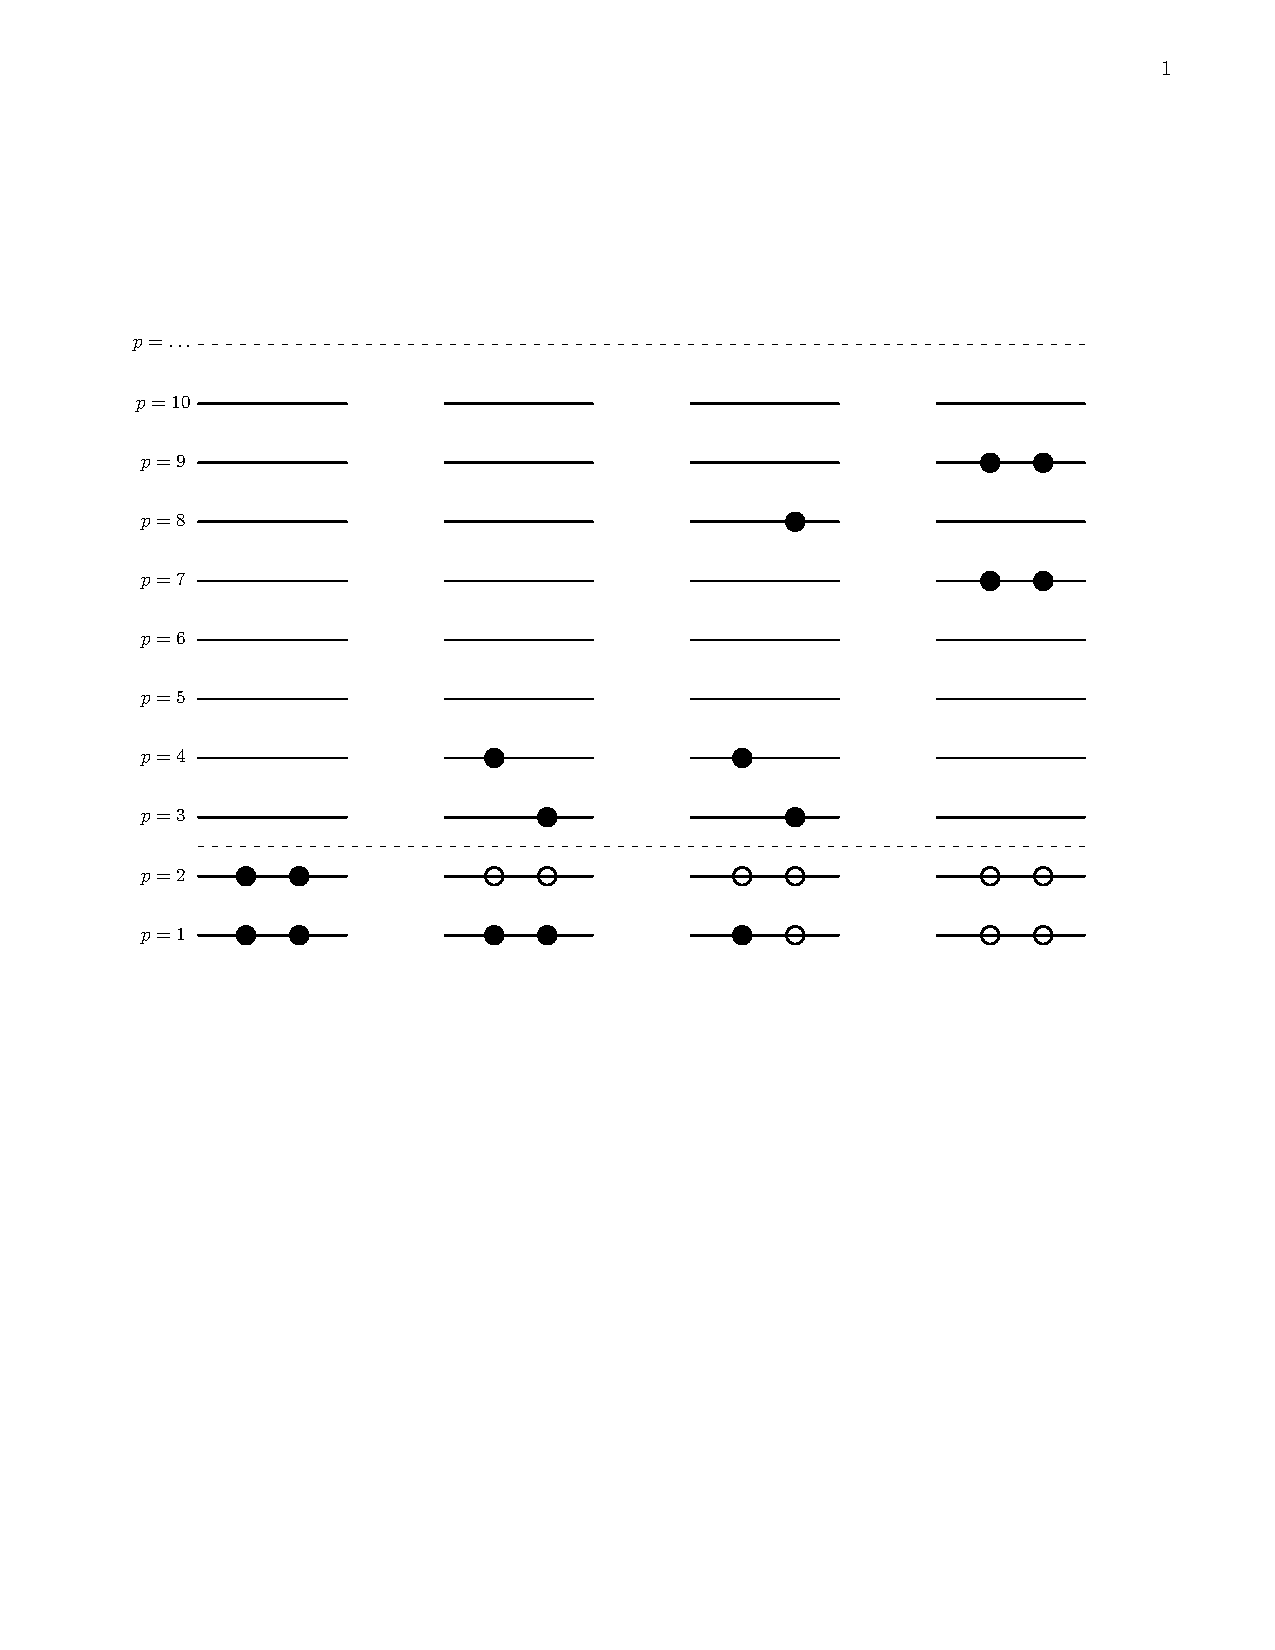
\includegraphics[width=0.7\textwidth]{figures/pairing/figpairing.pdf}
  \caption{Schematic plot of the possible single-particle levels with double degeneracy for four fermions.
The filled circles indicate occupied particle states while the empty circles 
represent vacant particle(hole) states.
The spacing between each level $p$ is constant in this picture. 
The first state to the left represents
a possible ground state representation for a four-fermion system. In the second state to the left,
one pair is broken by the interaction. 
All single-particle orbits belong to the model space. The two remaining four-particle states represents single-particle excitations to the excluded space, either by breaking two pairs or breaking one pair and exciting one pair (rightmost state). The latter two configurations cannot be produced by the pairing interaction alone. One would need to add an explicit pair-breaking term to the Hamiltonian.\label{fig:schematic}}
\end{figure}

Two exactly solvable cases play a central role in the benchmarks discussed in \cite{rigo2023} and reviewed here.
We distinguish between a so-called
\textbf{Constant-coupling pairing} with $g_{pq}=g$, giving
\begin{equation}
H=\sum_{p=1}^P d_p N_p - g\sum_{p,q=1}^P A_p^\dagger A_q,
\label{eq:H_const}
\end{equation}
with ground-state energies obtainable from Richardson equations \cite{Richardson:1963a,Richardson:1963b} (coupled nonlinear equations for pair energies). The next case is the so-called 
\textbf{Separable (hyperbolic) pairing}, with  a separable interaction with an energy cutoff $\alpha$,
\begin{equation}
H=\sum_{p=1}^P d_p N_p -2g\sum_{p,q=1}^P \sqrt{(\alpha-d_p)(\alpha-d_q)}\,A_p^\dagger A_q,
\label{eq:H_sep}
\end{equation}
which belongs to the hyperbolic Richardson-Gaudin family and is also
solvable by a related set of coupled equations.
These two approaches are used to assess the accuracy of our
network approaches beyond those model-spaces (defined by the
doubly-degenerate single-particle orbits $p$) that can be handled by
FCI theory.

Our variational Monte Carlo approach minimizes the Rayleigh--Ritz variational energy
\begin{equation}
E_V(\bm{\theta})=\frac{\bra{\psi_V(\bm{\theta})}H\ket{\psi_V(\bm{\theta})}}{\langle\psi_V(\bm{\theta})\vert\psi_V(\bm{\theta})\rangle},
\qquad E_0\le E_V(\bm{\theta}),
\label{eq:Ev}
\end{equation}
by varying the parameters $\bm{\theta}$ of a trial state $\ket{\psi_V}$.
In an occupation-number basis $\ket{\bm{n}}$ (here $\bm{n}=(n_1,\dots,n_p)$ with $n_p\in\{0,1\}$ indicating whether
a \emph{pair} occupies level $p$), the variational amplitudes are $\psi_V(\bm{n})=\braket{\bm{n}|\psi_V}$.
The configurations are sampled from
\begin{equation}
\mathbb{P}(\bm{n})\propto \vert\psi_V(\bm{n})\vert^2,
\label{eq:prob}
\end{equation}
and the energy estimator uses the local energy $E_L(\bm{n})$.
A practical advantage is that the occupation-number representation automatically encodes
fermionic antisymmetry/Pauli constraints, allowing comparatively simple NQS architectures. 
Our neural-network quantum state ansatz employs a real-valued NQS of the form
\begin{equation}
\psi_V(\bm{n})=e^{U(\bm{n})}\tanh\!\big(V(\bm{n})\big),
\label{eq:nqs}
\end{equation}
where $U$ and $V$ are fully connected feed-forward networks. In this parametrization, $U$ controls the magnitude,
while $\tanh(V)$ provides a smooth representation of the sign structure. In Ref.~\cite{rigo2023}, the author typically used two to three  hidden layers with
the $\tanh$-function as  activation function for the hidden layers. 

In the pairing Hamiltonian, off-diagonal contributions correspond to
moving a pair from an occupied level to an unoccupied one. For a given
configuration $\bm{n}$, only indices with $n_p=1$ and $n_q=0$
contribute, and the needed matrix elements can be computed by looping
over occupied/unoccupied sets and evaluating $\psi_V$ on the
configuration with $n_p\!\to 0$ and $n_q\!\to 1$. This structure keeps
the Monte Carlo evaluation efficient and explicitly tied to the
physical pair-scattering processes.

To optimize $\bm{\theta}$, stochastic reconfiguration  \cite{Sorella:2005} was applied, that is
\begin{equation}
S\,\delta\bm{\theta}=-\delta\tau\,\bm{G},
\label{eq:sr}
\end{equation}
where $\delta\tau$ is a step size, $S$ is an overlap/covariance matrix
of log-derivatives, and $\bm{G}$ is the energy gradient
estimator. Since the number of parameters grows with system size,
explicitly storing $S$ becomes prohibitive; we therefore solve
\eqref{eq:sr} with conjugate gradients, requiring only an efficient
routine for matrix-vector products $S\bm{v}$. To improve stability,
Rigo {\em et al.,} \cite{rigo2023} introduced a small diagonal
regularization inspired by RMSProp/Adam-style second-moment tracking
(with typical diagonal-shift strengths, see \cite{rigo2023} for additional information).

We have here, as done in Ref.~\cite{rigo2023}, chosen to present \emph{correlation energies} and benchmark the VMC--NQS method against exact diagonalization
(where feasible) and against two widely used approximations: many-body perturbation theory (MBPT) and pair coupled
cluster doubles excitations (pCCD). 

Figure \ref{fig:corr_constant} demonstrates the optimization dynamics for the constant-coupling pairing Hamiltonian
\eqref{eq:H_const} with $P=10$ levels and $M=5$ pairs. The plotted observable is the correlation energy
as function of the strength of the pairing interaction.
\begin{figure}[hbtp]
    \centering
    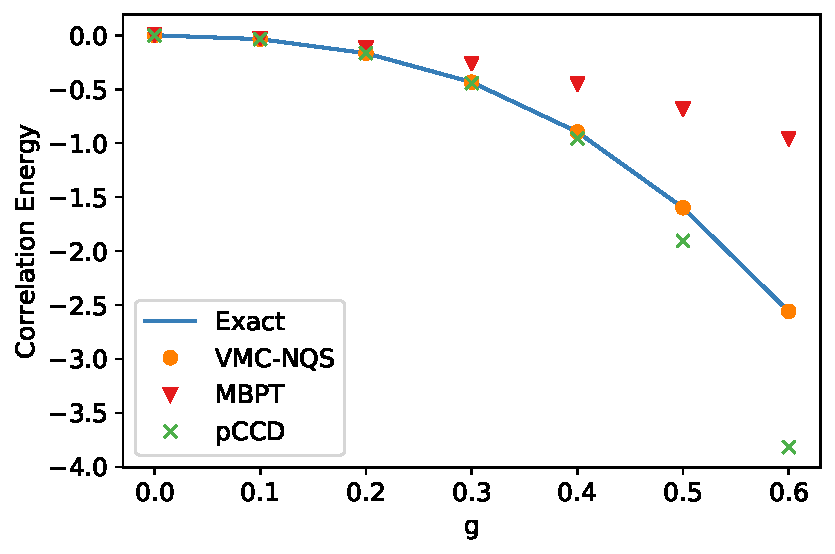
\includegraphics[width=0.8\textwidth]{figures/pairing/g_constant_energies.pdf}
    \caption{Correlation energy for the constant-coupling model for $P=10$ single-particle energy levels and $M=5$ pairs as a function of the interaction strength. VMC-NQS (solid orange circles), MBPT (solid red triangles), and pCCD (green crosses) calculations are compared with the exact answer (solid line). Taken from \cite{rigo2023}.}
    \label{fig:corr_constant}
\end{figure}
After roughly $10^3$ optimization steps, the VMC--NQS correlation energy converges to the exact-diagonalization
value. the final precision level is around $10^{-7}$ in the converged correlation energy.
In this figure, three approximations (MBPT, pCCD, VMC--NQS) are plotted against the exact
result. We note from this figure that 
\begin{itemize}
\item \textbf{Weak coupling:} all methods agree closely at small $\vert g\vert$, consistent with perturbative expectations. 
\item \textbf{MBPT breakdown:} deviations from exact diagonalization become visible already around $g\approx \vert 0.2\vert$. This is interpreted as the inability of low-order perturbation theory to capture
nonperturbative pairing correlations at stronger coupling. 
\item \textbf{pCCD: initially robust, then overbinding:} pCCD remains closer down to about $g\approx \vert 0.4\vert$ but becomes
significantly \emph{too low} for more negative $g$, that is it overbinds and thereby violates the variational principle.
\item \textbf{VMC--NQS: uniform accuracy and variational safety:} VMC--NQS tracks the exact curve across the full range
shown, with discrepancies remaining below $10^{-4}$.
\end{itemize}

The main methodological message of Fig.~\ref{fig:corr_constant} is
that enforcing a \emph{variational} optimization over a flexible NQS
ansatz yields a solver that remains reliable precisely where MBPT and
pCCD lose quantitative control.


The authors of Ref.~\cite{rigo2023}  extended the comparative analysis by considering a larger model
space, with up to $P=40$ energy levels and $M=20$ pairs of
fermions. In Table~\ref{tab:g_constant_large}, we list here  the
correlation energies obtained within VMC-NQS, pCCD, and the
highly-accurate iterative approach for solving the Richardson
equations developed in Ref.~\cite{Guan:2022CoPhC}. To make contact
with the results of the latter reference, the single-particle energies
are re-scaled as $d_p = p / 10$ and the pairing strength is taken to
be $g=-0.05$. Similarly to the smaller model space, the correlation
energies computed within VMC-NQS are almost always in perfect
agreement with the ones obtained from the Iterative method. The only
exception is the case with $P=40$ and $M=20$, for which the VMC-NQS
yields $-1.785$, while the iterative method provides $-2.111$.  On
the other hand, pCCD struggles already for $P=10$ and $M=5$, where it
yields $\sim 20\%$ overbinding. Increasing the number of
single-particle states and pairs, pCCD becomes more and more
unreliable, with large departures from both the exact and VMC-NQS
values. This behavior is due to the the pairing interaction terms
growing faster with the number of states than the mean-field one,
making the exact ground-state very different from the Hartree-Fock
solution.

\begin{table}[hbtp]
\begin{center}
\vspace{0.5cm}
\begin{tabular}{ c | c | c c c c }
\hline
\hline
& $P$ & $M=5$  & $M=10$ & $M=15$ & $M=20$ \\
\hline
VMC-NQS & \multirow{3}{*}{ 10 }  & -0.160 & 0.000 & - & - \\
pCCD &  & -0.193 & 0.000 & - &  -\\
Iterative &  & -0.160  & 0.000 & - & - \\
\hline
VMC-NQS & \multirow{3}{*}{ 20 }  & -0.394 & -0.515 & -0.394 & 0.000 \\
pCCD &   & -0.987 & -1.743 & -1.110 &  0.000 \\
Iterative &   & -0.394 & -0.515 & -0.394 &  0.000 \\
\hline
VMC-NQS & \multirow{3}{*}{ 30 }  & -0.606 & -0.946 & -1.057 & -0.946 \\
pCCD &   & -1.750 & 3.500 & -6.467 &  -5.697\\
Iterative &   & -0.606 & -0.946 & -1.057 & -0.946\\
\hline
VMC-NQS & \multirow{3}{*}{ 40 }  & -0.809 & -1.356 & -1.678 & -1.785 \\
pCCD &   & -4.231 & 124.923 & 7.598 &  -44.346 \\
Iterative &   & -0.809 & -1.356 & -1.678 & -2.110\\
\hline
\end{tabular}
\caption{Correlation energies obtained with the VMC-NQS method compared with pCCD and the iterative approach of Ref.~\cite{Guan:2022CoPhC} for the constant-coupling Hamiltonian of Eq.~\eqref{pairing_model_hamiltonian_constant_g} with $g = 0.05$ and $d_p=p/10$. Taken from Ref.~\cite{rigo2023}.}
\label{tab:g_constant_large}
\end{center}
\end{table}

These results establish that a variational Monte Carlo approach  in an occupation-number basis with a
compact NQS ansatz can solve integrable nuclear pairing Hamiltonians
with near-exact accuracy over a wide coupling range, while maintaining
the variational bound by construction. The Stochastic Reconfiguration together with the RMSProp update of the learning rates
provide stable convergence, and the benchmarks against exact
diagonalization show that VMC--NQS remains accurate where MBPT and
pCCD deviate or violate variationality. The authors also report on
broader tests and argue that the approach exhibits polynomial scaling
in $P$, motivating extensions to nonseparable, state-dependent pairing
interactions and to larger shell-model Hamiltonians where exact
diagonalization is infeasible due to too large dimensionalities.







